\section{Deep Networks Models}
\label{sec:models}

This section describes and compare the original model proposed by the TensorFlow\textsuperscript{TM} tutorial and three possible modifications.
All network are initialized using the same seed for random number generation in order to obtain results with are comparable.
Also the selection of the initial subsets of the training and test sets are done with the same fixed seed.


\subsection{Original Model}

The original network proposed has the following architecture:
a Convolutional layer, a Pooling layer, another Convolutional layer, another Pooling layer, a Fully Connected layer with \ac{ReLU} activation function and Dropout and a Softmax output layer.
The first Convolutional layer computes 32 filters, while the second one 64.
Both Pooling layers reduces the dimension of the image by applying max pooling with 2x2 pixel patches and stride 2.
\cref{fig:graph} shows the structure of the resulting network.

\begin{figure}[t]
	\centering
	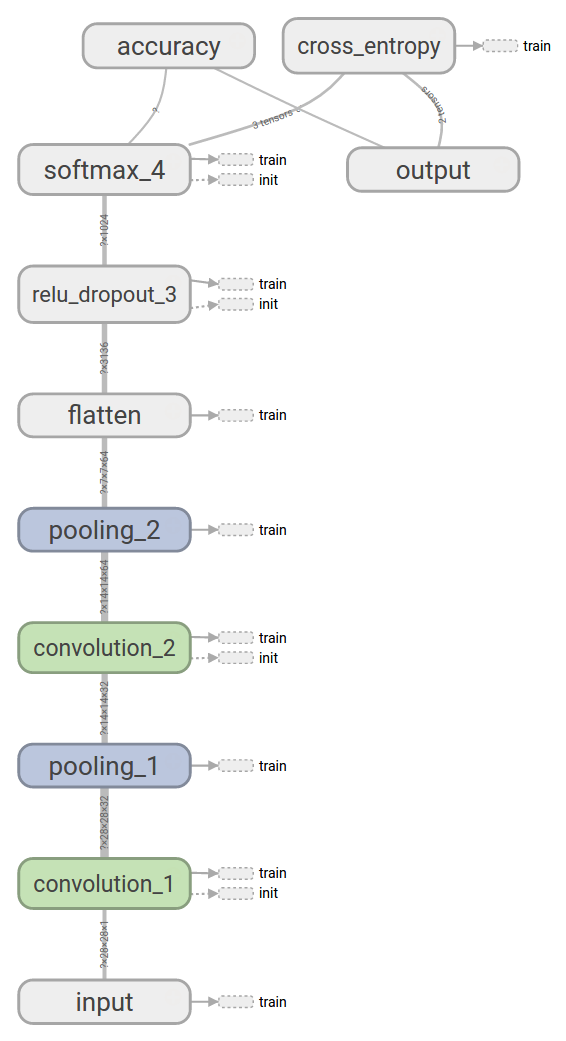
\includegraphics[width=\columnwidth]{figures/graph}
	\caption{Structure of the original Deep Network used for the MNIST handwritten digits recognition, visualized using the TensorBoard tool.}
	\label{fig:graph}
\end{figure}

The Convolutional layers are used to extract features from the images, which are then used by the Fully Connected layer and the Softmax layer to compute the most probable class.
Pooling layers and Dropout are used to prevent the network to overfit the training data.
Note that the image is reshaped into a one dimensional array after the second Pooling layer, in order to be processed by the Fully Connected layer.

At each training step, the network is trained with a batch of 50 images, randomly selected from the train dataset.
The network is trained to minimize the generalized cross entropy function for a multiclass problems.
After 20000 epochs of training, the network has an accuracy of $99.17\%$ on the complete test set.
It is not clear if the accuracy could get better with more training, since its accuracy over time is not stable (see \cref{fig:performances}).

\begin{figure}[t]
	\centering
	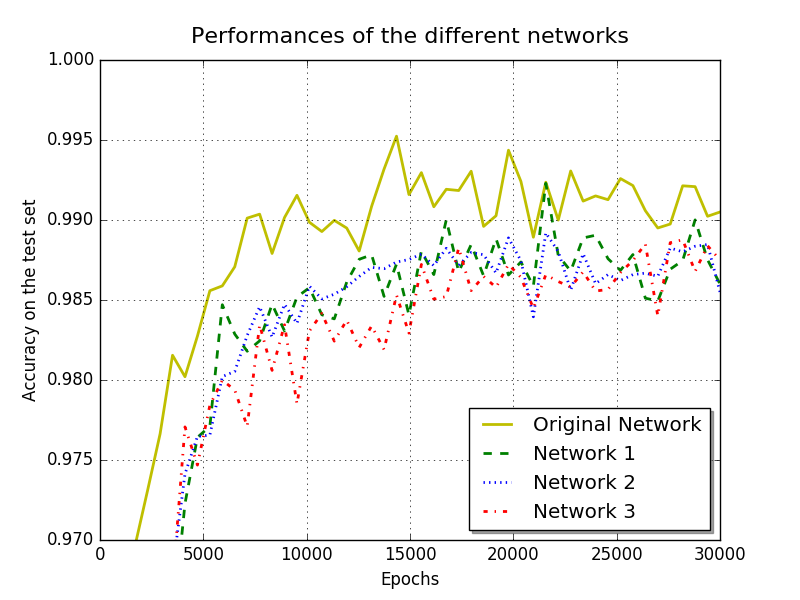
\includegraphics[width=\columnwidth]{figures/performances}
	\caption{The graph shows the performances of the different networks on the test set over epochs of training. The plotted accuracies are measured on a random fixed subset of $1000$ elements of the test set, equal for all the networks.}
	\label{fig:performances}
\end{figure}


\subsection{Model 1}

The first modification to the original model consist in removing the first level of Convolution and Pooling.
The second Convolutional layer is now directly applied to the original image.
The rest of the network and all hyperparameters are unchanged.

The performance of the network is closed to the original one, with an accuracy of $98.99\%$ on the test set.
As for the original model, it is not clear whether the accuracy could increase with more training. 


\subsection{Model 2}

The second modification is very similar to the previous one. Instead of removing the first one, we are removing the second Convolution and Pooling layers.
The resulting network is almost identical to Model 1, but with the difference that the layer is computing 32 filters instead of 64.
The accuracy of this model is $98.94\%$.


\subsection{Model 3}

The third moditifaction consist in removing the Fully Connected layer.
The accuracy of this network is slighly worse then the other models and scores $98.89\%$.
This is probably due to the absence of any fully connected layer that properly combines the features extracted by the convolutional layer.
Like for the other networks, it is not clear if the performances can improve with more training.
